\chapter{复变函数}

\section{复变函数的概念}

\subsection{复变函数的定义}

复变函数 $f $ 是黎曼面 $\mathbb{C}^\mathrm{R} $ 到复平面 $\mathbb{C} $ 的映射。

\section{解析函数}

\subsection{复变函数的连续性}

设复变函数 $f(z)$ 在 $z_0$ 点及其邻域内有定义。当自变量 $z$ 以任何路径趋于 $z_0$ 时,都有

\begin{equation}
\lim_{z\to z_0} f(z)
=f(z_0),
\end{equation}

则称 $f(z)$ 在 $z_0$ 点连续。

若 $f(z)$ 在区域 $\Omega$ 内的所有点都连续,则称 $f(z)$ 在 $\Omega$ 内连续。

\subsection{复变函数的导数}

设 $z_0 $ 是复变函数 $f(z) $ 定义域 $\Omega $ 内的一点。当 $z$ 以任何路径趋于 $z_0$ 时,即 $\Delta z=z-z_0$ 以任何方式趋于 $0$ 时,若极限

\begin{equation}
\lim_{\Delta z\to 0}\frac{f(z_0+\Delta z)-f(z_0)}{\Delta z}
\end{equation}

存在且唯一,则称 $f(z)$ 在 $z_0$ 点可导,$f(z)$ 在 $z_0$ 点的导数记为 $f'(z_0).$

\subsection{柯西-黎曼条件}

\begin{theorem}

设复变函数 $f(z)=u(x,y)+\mathrm{i}v(x,y)$,若 $f(z)$ 在 $z$ 点可导,则必定有:

\begin{equation}
\frac{\partial u}{\partial x}
=\frac{\partial v}{\partial y},\quad
\frac{\partial u}{\partial y}
=-\frac{\partial v}{\partial x}.
\end{equation}

上面两条等式称为柯西-黎曼条件(C-R条件)。

\end{theorem}

\begin{proof}

设 $z=x+\mathrm{i} y,f(z)=u(x,y)+\mathrm{i}v(x,y)$,则:

\begin{equation}
\lim_{\Delta z\to 0} \frac{f(z+\Delta z)-f(z)}{\Delta z}
=\lim_{\Delta z\to 0}\frac{\Delta u+\mathrm{i}\Delta v}{\Delta x+\mathrm{i}\Delta y}.
\end{equation}

由于 $f(z)$ 在 $z$ 点可导,故极限

\begin{equation}
\lim_{\Delta z\to 0} \frac{f(z+\Delta z)-f(z)}{\Delta z}
\end{equation}

存在且与 $\Delta z$ 趋于 $0$ 的方式无关。

特别地,

(1)令

\begin{equation}
\mathrm{i}\Delta y=0,\quad \Delta x\to 0,
\end{equation}

此时

\begin{equation}
\lim_{\Delta z\to 0}\frac{\Delta u+\mathrm{i}\Delta v}{\Delta x+\mathrm{i}\Delta y}
=\lim_{\Delta x\to 0}\frac{\Delta u+\mathrm{i}\Delta v}{\Delta x}
=\frac{\partial u}{\partial x}+\mathrm{i}\frac{\partial v}{\partial x}.
\end{equation}

(2)令

\begin{equation}
\Delta x=0,\quad\mathrm{i}\Delta y\to 0,
\end{equation}

此时

\begin{equation}
\lim_{\Delta z\to 0}\frac{\Delta u+\mathrm{i}\Delta v}{\Delta x+\mathrm{i}\Delta y}
=-\mathrm{i}\frac{\partial u}{\partial y}+\frac{\partial v}{\partial y}.
\end{equation}

由于 $f(z)$ 在 $z_0$ 点可导,则这两个导数值应该相等,对比实部和虚部就得到

\begin{equation}
\frac{\partial u}{\partial x}
=\frac{\partial v}{\partial y},\quad
\frac{\partial u}{\partial y}
=-\frac{\partial v}{\partial x}.
\end{equation}

\end{proof}

C-R 条件是 $f(z) $ 在 $z $ 点可导的必要条件,但不是充分条件。也就是说,可导必定满足 C-R 条件,但满足 C-R 条件不一定可导。

\subsection{解析函数的定义}

若复变函数 $f(z)$ 在 $z_0$ 的邻域内每一点都可导,则称 $f(z)$ 在 $z_0$ 点是解析的。

若复变函数 $f(z)$ 在 $\Omega$ 内每一点都可导,则称 $f(z)$ 在 $\Omega$ 内是解析的,或称为全纯的。

\subsection{例题}

\begin{example}
    
已知解析函数 $f(z)=u+\mathrm{i}v $ 的实部 $u=x^3-3xy^2 $,求该解析函数。

\end{example}

\begin{solution}
    
解析函数应满足柯西-黎曼条件:

\begin{equation}
\frac{\partial u}{\partial x}
=\frac{\partial v}{\partial y},\quad
\frac{\partial u}{\partial y}
=-\frac{\partial v}{\partial x},
\end{equation}

\begin{equation}
\frac{\partial v}{\partial y}
=\frac{\partial u }{\partial x } 
=3x^2-3y^2,\quad
\frac{\partial v}{\partial x}
=-\frac{\partial u }{\partial y } 
=6xy,
\end{equation}

\begin{equation}
\mathrm{d}v(x,y)
=\frac{\partial v }{\partial x }\mathrm{d}x + \frac{\partial v }{\partial y } \mathrm{d}y
=6xy\mathrm{d}x+\left(3x^2-3y^2\right)\mathrm{d}y.
\end{equation}

选择积分路径为:$\underbrace{(0,0)\to(x_0,0)}_{C_1},\underbrace{(x_0,0)\to(x_0,y_0)}_{C_2}$,在路径 $C_1 $ 上有 $y=0,\mathrm{d}y=0 $,在路径 $C_2 $ 上有 $x=x_0,\mathrm{d}x=0 $,两边积分:

\begin{equation}
\begin{split}
v(x_0,y_0)-v(0,0)
&=\int\limits_{C_1} 6xy\mathrm{d}x + \left(3x^2-3y^2\right)\mathrm{d}y + \int\limits_{C_2}6xy\mathrm{d}x + \left(3x^2-3y^2\right)\mathrm{d}y \\
&=0+\int_{y=0}^{y=y_0}\left(3x_0^2-3y^2\right)\mathrm{d}y \\
&=3x_0^2 y_0-y_0^3.
\end{split}
\end{equation}

令 $v(0,0)=C$,则:

\begin{equation}
v(x,y)
=3x^2y-y^3+v(0,0)
=3x^2y-y^3+C,
\end{equation}

于是:

\begin{equation}
\begin{split}
f(z)
&=u(x,y)+\mathrm{i}v(x,y) \\
&=x^3-3xy^2+\mathrm{i}\left(3x^2 y-y^3+C\right).
\end{split}
\end{equation}

\end{solution}

\begin{example}
    
已知解析函数 $f(z)=u + \mathrm{i} v $ 的虚部 $\displaystyle{v=\frac{y }{x^2+y^2 }  }$,求该解析函数。

\end{example}

\begin{solution}

先计算偏微分:

\begin{equation}
\frac{\partial v}{\partial x}
=\frac{-2xy}{\left(x^2+y^2\right)^2},\quad
\frac{\partial v}{\partial y}
=\frac{x^2-y^2}{\left(x^2+y^2\right)^2},
\end{equation}

函数解析,故满足 C-R 条件,即满足:

\begin{equation}
\frac{\partial u}{\partial x}
=\frac{\partial v }{\partial y } 
=\frac{x^2-y^2}{\left(x^2+y^2\right)^2},
\end{equation}

\begin{equation}
\frac{\partial u}{\partial y}
=-\frac{\partial v }{\partial x } 
=\frac{2xy}{\left(x^2+y^2\right)^2},
\end{equation}

于是:

\begin{equation}
\mathrm{d}u
=\frac{\partial u }{\partial x } \mathrm{d}x + \frac{\partial u }{\partial y } \mathrm{d}y
=\frac{x^2-y^2}{\left(x^2+y^2\right)^2}\mathrm{d}x+\frac{2xy}{\left(x^2+y^2\right)^2}\mathrm{d}y,
\end{equation}

看到 $\left(x^2+y^2 \right) $,很自然想到极坐标变换:

\begin{equation}
\left\{
\begin{aligned}
&x=\rho\cos\varphi \\
&y=\rho\sin\varphi
\end{aligned}
\right.
\Longrightarrow
\left\{
\begin{aligned}
&\mathrm{d}x = \frac{\partial x }{\partial \rho } \mathrm{d}\rho + \frac{\partial x }{\partial \varphi } \mathrm{d}\varphi = \cos\varphi\mathrm{d}\rho - \rho \sin\varphi \mathrm{d}\varphi \\
&\mathrm{d}y = \frac{\partial y }{\partial \rho } \mathrm{d}\rho + \frac{\partial y }{\partial \varphi } \mathrm{d}\varphi = \sin\varphi \mathrm{d}\rho + \rho\cos\varphi \mathrm{d}\varphi
\end{aligned}
\right. ,
\end{equation}

于是:

\begin{equation}
\begin{split}
\mathrm{d}u
&=\frac{x^2-y^2}{\left(x^2+y^2\right)^2}\mathrm{d}x+\frac{2xy}{\left(x^2+y^2\right)^2}\mathrm{d}y \\
&=\frac{\cos\varphi }{\rho^2 } \mathrm{d}\rho + \frac{\sin\varphi }{\rho } \mathrm{d}\varphi \\
&=\mathrm{d}\left(\frac{-\cos\varphi }{\rho }  \right),
\end{split}
\end{equation}

于是:

\begin{equation}
u
=\frac{-\cos\varphi }{\rho } + C
=-\frac{x }{x^2+y^2 } + C,
\end{equation}

综上,

\begin{equation}
\begin{split}
f(z)
&=u + \mathrm{i} v \\
&=\left(-\frac{x }{x^2+y^2 } + C \right) + \mathrm{i}\left(\frac{y }{x^2+y^2 } \right).
\end{split}
\end{equation}

\end{solution}

\section{复变函数积分}

\subsection{复变函数积分的定义}

复变函数的积分是指复变函数 $f(z)$ 在其有定义的区域中,沿某一曲线 $C$ 的有向的线积分。

复变函数 $f(z) $ 沿曲线 $C $ 的积分,记为 $\displaystyle{\int\limits_{C} f(z)\mathrm{d}z }$,由下式定义:

\begin{equation}
\int\limits\limits_C f(z)\mathrm{d}z
\equiv \lim\limits_{\substack{n\to \infty \\ |z_j-z_{j-1}|\to 0 }}\sum\limits_{j=1}^{n} f(\xi_j) (z_j-z_{j-1}).
\end{equation}

右边的东西就是说,$C $ 分成 $n $ 段,每段都很短,端点记为 $z_0,z_1,\cdots,z_n $,$\xi_j $ 是 $C $ 上 $z_{j-1} $ 点到 $z_j $ 点的中的某一点,最后再令 $n $ 趋于无穷。

\subsection{柯西积分定理}

\subsubsection{单连通区域柯西积分定理}

设 $f(z)$ 在单连通区域(内部没有洞的区域) $\Omega$ 上解析,当积分路径为 $\Omega$ 内的任一闭合曲线 $C$ 时,有: 

\begin{equation}
\oint\limits_{C^+} f(z)\mathrm{d}z
=0.
\end{equation}

其中,$\displaystyle{\oint\limits_{C^+} }$ 代表积分沿闭合曲线 $C $ 的逆时针方向进行。

\subsubsection{多连通区域柯西积分定理}

设 $f(z)$ 在具有 $k$ 个内边界 $C_1,C_2,\cdots,C_k$ 的回路 $C$ 内的多连通区域内解析,规定 $C,C_1,C_2,\cdots,C_k $ 的正方向为逆时针,则:

\begin{equation}
\oint\limits_{C^+} f(z)\mathrm{d}z
=\oint\limits_{C_1^+} f(z)\mathrm{d}z+\oint\limits_{C_2^+} f(z)\mathrm{d}z+\cdots+\oint\limits_{C_k^+} f(z)\mathrm{d}z.
\end{equation}

\subsection{柯西积分公式}

若 $f(z)$ 在闭合回路 $C$ 所包围的区域上解析,$z_0$ 是此区域中的一点,则:

\begin{equation}
\oint\limits_{C^+}\frac{f(z)}{z-z_0}\mathrm{d}z
=2\pi \mathrm{i} f(z_0).
\end{equation}

\subsection{解析函数高阶导数的积分表达式}

设 $f(z)$ 在区域 $\Omega$ 内解析,$C$ 为 $\Omega$ 内的任一闭合回路,对于 $C$ 所包围的区域内的任一点 $z$,有:

\begin{equation}
f^{(n)}(z)
\equiv \frac{\mathrm{d}^n }{\mathrm{d}z^n }f(z) 
=\frac{n!}{2\pi\mathrm{i}}\oint\limits_{C^+} \frac{f(\zeta)}{(\zeta-z)^{n+1}}\mathrm{d}\zeta.
\end{equation}

\section{复变函数的级数展开}

\subsection{解析函数的泰勒展开}

设 $z_0$ 为函数 $f(z)$ 解析区域 $\Omega$ 内的一点,以 $z_0$ 为圆心的圆周 $C$ 在 $\Omega$ 内,则 $f(z)$ 可以在 $C$ 内展成泰勒级数:

\begin{equation}
f(z)
=\sum_{n=0}^{\infty} a_n(z-z_0)^n,
\end{equation}

其中,展开系数为:

\begin{equation}
a_n
=\frac{f^{(n)}(z_0)}{n!}
=\frac{1}{2\pi \mathrm{i}}\oint\limits_{C^+} \frac{f(z)}{(z-z_0)^{n+1}}\mathrm{d}z.
\end{equation}

\subsection{解析函数的洛朗展开}

\subsubsection{复变函数的零点}

若复变函数 $f(z) $ 在 $z_0 $ 点的函数值 $f(z_0)=0 $,则称 $z_0 $ 为复变函数 $f(z) $ 的零点。

\subsubsection{复变函数的奇点}

若复变函数 $f(z) $ 在 $z_0 $ 点不解析,即 $f(z) $ 在 $z_0 $ 点的导数不存在或不唯一,则称 $z_0 $ 为复变函数 $f(z) $ 的奇点。

\subsubsection{奇点的分类}

\begin{itemize}
    \item 孤立奇点:若 $z_0$ 为函数 $f(z)$ 的奇点,而在 $z_0$ 点任意小的邻域内,函数 $f(z)$ 解析,则称 $z_0$ 为 $f(z)$ 的孤立奇点。
    \item 非孤立奇点:若 $z_0$ 为函数 $f(z)$ 的奇点,而在 $z_0$ 点任意小的邻域内,除 $z_0 $ 点外存在 $f(z) $ 的其他奇点,则称 $z_0$ 为 $f(z)$ 的非孤立奇点。
\end{itemize}

还可以进一步对孤立奇点分类。

\begin{itemize}
    \item 极点:设 $z_0$ 是 $f(z)$ 的孤立奇点,若存在一个正整数 $k$,使得 $(z-z_0)^kf(z)$ 为非零的解析函数,则称 $z_0$ 为 $f(z)$ 的 $k$ 阶极点。
    \item 本性奇点:设 $z_0$ 是 $f(z)$ 的孤立奇点,若不存在一个正整数 $k$,使得 $(z-z_0)^kf(z)$ 为非零的解析函数,则称 $z_0$ 为 $f(z)$ 的本性奇点。
    \item 可去奇点:设 $z_0$ 为函数 $f(z)$ 的孤立奇点,$f(z)$ 在 $z_0$ 点没有定义,但在 $z_0$ 的去心邻域内解析,此时可定义 $f(z_0)\equiv \lim\limits_{z\to z_0} f(z)$ 使 $f(z)$ 在 $z_0$ 点解析,则称 $z_0$ 为 $f(z)$ 的可去奇点。
\end{itemize}

\subsubsection{解析函数的洛朗展开}

若函数 $f(z)$ 在以 $z_0$ 为圆心,半径为 $R_1,R_2$ 的两个圆周 $C_1,C_2$ 所包围的环形区域 $R_2<|z-z_0|<R_1$ 上解析,则在此区域内 $f(z)$ 可展成 Laurent 级数:

\begin{equation}
f(z)
=\sum_{n=-\infty}^{\infty}a_n(z-z_0)^n,
\end{equation}

其中,

\begin{equation}
a_n
=\frac{1}{2\pi \mathrm{i}}
\oint\limits_{C^+}\frac{f(\zeta)}{(\zeta-z_0)^{n+1}}\mathrm{d}\zeta.
\end{equation}

$C$ 是任一条在环形区域内把 $C_2$ 包围在内的闭曲线。

\subsection{例题}

\begin{example}
    
求 $\displaystyle{f(z)=\frac{1 }{z(z-1) }  }$ 在环形区域 $0<|z|<1 $ 和 $|z|>1 $ 内,在 $z_0=0 $ 处的展开式。

\end{example}

\begin{solution}
    
首先想到几何级数:

\begin{equation}
\frac{1 }{1-z } 
=\sum_{n=0}^{\infty} z^n,\quad \left|z \right|<1.
\end{equation}

把 $f(z) $ 拆分:

\begin{equation}
\begin{split}
f(z)
&=\frac{1}{z(z-1)} \\
&=\frac{z - (z-1)}{z(z-1) }  \\
&=\frac{1}{z-1}-\frac{1}{z} \\
&=\frac{1}{z-1}-z^{-1}.
\end{split}
\end{equation}

当 $\left|z \right|<1 $ 时,有

\begin{equation}
\begin{split}
f(z)
&=\frac{1}{z-1}-z^{-1} \\
&=- \frac{1 }{1-z } - z^{-1} \\
&=-\left(\sum_{n=0}^{\infty} z^n \right) - z^{-1} \\
&=\sum_{n=-1}^{\infty} (-1) z^n .
\end{split}
\end{equation}

当 $\left|z \right|>1 $ 时,注意到 $|1/z|<1 $,于是:

$$
\begin{aligned}
f(z)
&=\frac{1}{z-1}-z^{-1} \\
&=\frac{1}{z(1-\frac{1}{z})}-z^{-1} \\
&=\frac{1}{z}\cdot \frac{1}{1-\frac{1}{z}} -z^{-1} \\
&=\frac{1}{z}\sum_{n=0}^{\infty} \left(\frac{1}{z}\right)^{n}-z^{-1} \\
&=\sum_{n=0}^{\infty} z^{-n-1}-z^{-1} \\
&=\sum_{n=1}^{\infty} z^{-n-1}.
\end{aligned}
$$

\end{solution}

\begin{example}
    
求 $\displaystyle{f(z)=\frac{1 }{z(z-1) }  }$ 在 $z_1=0 $ 和 $z_2=1 $ 附近的展开式。

\end{example}

\begin{solution}
    
先算 $f(z) $ 在 $z_1=0 $ 附近的展开式。

由于 $0<|z-0|<1 $,于是:

\begin{equation}
\begin{split}
f(z)
&=\frac{1}{z(z-1)} \\
&=\frac{1}{z-1}-\frac{1}{z} \\
&=-\frac{1}{1-z}-z^{-1} \\
&=-\sum_{n=0}^{\infty} z^n-z^{-1} \\
&=\sum_{n=-1}^{\infty} (-1)z^n.
\end{split}
\end{equation}

再算 $f(z) $ 在 $z_2=1 $ 附近的展开式。

由于 $0<|z-1|<1 $,于是:

\begin{equation}
\begin{split}
f(z)
&=\frac{1}{z(z-1)} \\
&=\frac{1}{z-1}-\frac{1}{z} \\
&=(z-1)^{-1} - \frac{1 }{1-(1-z) } \\
&=(z-1)^{-1} - \sum_{n=0}^{\infty} (1-z)^n \\
&=(z-1)^{-1} - \sum_{n=0}^{\infty} \left(-1 \right)^n (z-1)^n \\
&=(z-1)^{-1} + \sum_{n=0}^{\infty} \left(-1 \right)^{n+1} (z-1)^n \\
&=\sum_{n=-1}^{\infty} \left(-1 \right)^{n+1} (z-1)^n.
\end{split}
\end{equation}

\end{solution}

\section{留数定理及其应用}

\subsection{留数的定义}

设 $z_0$ 是函数 $f(z)$ 的孤立奇点,设 $f(z)$ 在其孤立奇点 $z_0$ 附近的环形区域中的洛朗展开式为:

\begin{equation}
f(z)
=\sum\limits_{n=-\infty}^{\infty} a_n(z-z_0)^n .
\end{equation}

$f(z)$ 在 $z_0$ 点的留数,记为 $\mathrm{Res}f(z_0)$,定义为:

\begin{equation}
\mathrm{Res} f(z_0)
\equiv a_{-1},
\end{equation}

其中,$a_{-1}$ 是 $f(z)$ 在 $z_0$ 点的洛朗展开式中 $(z-z_0)^{-1}$ 项的系数。

\subsection{留数的求法}

\subsubsection{定义法}

直接把 $f(z)$ 在其孤立奇点 $z_0$ 点作洛朗展开:

\begin{equation}
f(z)
=\sum\limits_{n=-\infty}^{\infty} a_n(z-z_0)^n,
\end{equation}

找到 $(z-z_0)^{-1}$ 前的系数 $a_{-1}$,由留数的定义可知:

$$
\mathrm{Res} f(z_0)\equiv a_{-1}.
$$

\subsubsection{极限法}

当 $z_0$ 为 $f(z)$ 的 $m$ 阶极点时,$f(z)$ 可在其孤立奇点 $z_0$ 点作如下的洛朗展开:

\begin{equation}
f(z)
=\sum_{n=-m}^{\infty} a_n(z-z_0)^n,~~a_{-m}\ne 0,
\end{equation}

则

\begin{equation}
\mathrm{Res}f(z_0)
=\frac{1}{(m-1)!}\lim_{z\to z_0}\frac{\mathrm{d}^{m-1}}{\mathrm{d}z^{m-1}}[(z-z_0)^mf(z)].
\end{equation}

\subsubsection{特殊情况}

若 $f(z)=\frac{h(z)}{g(z)},z_0$ 为 $g(z)$ 的一阶极点,且 $h(z)$ 和 $g(z)$ 在 $z_0$ 点及其邻域内解析,则:

\begin{equation}
\mathrm{Res}
f(z_0)
=\frac{h(z_0)}{g'(z_0)}.
\end{equation}

\subsection{留数定理}

若 $f(z)$ 在回路 $C$ 所包围的区域内除有限个孤立奇点 $z_1,z_2,\cdots,z_k$ 外解析,则 $f(z)$ 沿 $C^+$ 的回路积分值等于 $f(z)$ 在 $z_1,z_2,\cdots,z_k$ 的留数之和乘 $2\pi\mathrm{i}$,即:

$$
\oint\limits_{C^+} f(z)\mathrm{d}z
=2\pi\mathrm{i}\sum\limits_{j=1}^{k} \mathrm{Res} f(z_j).
$$

\subsection{利用留数定理求无穷级数}

\subsubsection{所需函数}

\begin{figure}[h]
\centering
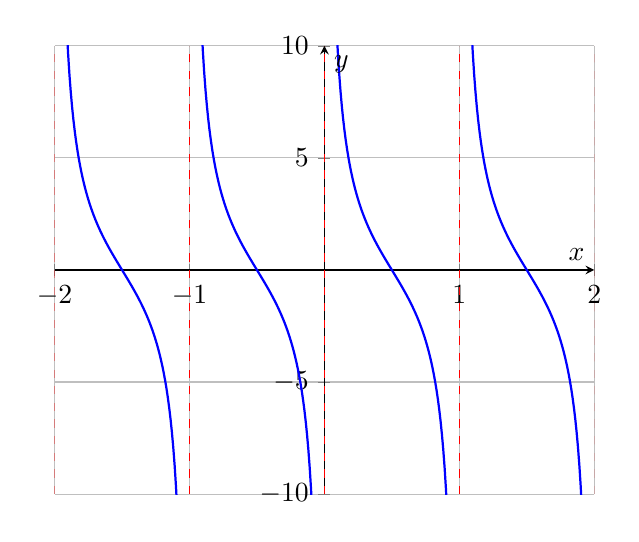
\begin{tikzpicture}
\begin{axis}[
    axis lines = middle,
    xlabel = {$x$},
    ylabel = {$y$},
    xmin=-2, xmax=2,
    ymin=-10, ymax=10,
    xtick={-2,-1,0,1,2},
    ytick={-10,-5,0,5,10},
    grid=both,
]

% 分段绘制 pi * cot(pi x),避开整数点
\addplot[blue, thick, samples=100, domain=-2:-1.01] {pi*cot(deg(pi*x))};
\addplot[blue, thick, samples=100, domain=-0.99:-0.01] {pi*cot(deg(pi*x))};
\addplot[blue, thick, samples=100, domain=0.01:0.99] {pi*cot(deg(pi*x))};
\addplot[blue, thick, samples=100, domain=1.01:2] {pi*cot(deg(pi*x))};

% 竖直虚线表示整数点渐近线
\foreach \x in {-2,-1,0,1,2}
    \addplot[red, dashed] coordinates {(\x,-10) (\x,10)};

\end{axis}
\end{tikzpicture}
\caption{Plot of $y = \pi \cot (\pi x)$ with vertical asymptotes at integers.}
\label{fig:cotplot}
\end{figure}

\subsubsection{例题}

\begin{example}
    
计算 $\displaystyle{\sum_{n=1}^{\infty} \frac{1 }{n^2-a^2 }  }$,其中 $a>0,a\notin \mathbb{Z} .$

\end{example}

\begin{solution}
    
为了计算目标无穷级数,考虑如下的无穷级数:$\displaystyle{\sum_{n=-\infty}^{\infty} \frac{1 }{n^2-a^2 }  }$,其中 $a>0,a\notin \mathbb{Z} .$

构造函数 $\displaystyle{f(z)=\pi \cot (\pi z) \cdot \frac{1 }{z^2-a^2 }  }$,由 $\pi \cot(\pi z) $ 的性质可知,$f(z) $ 的全部奇点 $z_\pm = \pm a,z_i = i\in\mathbb{Z} $ 都是一阶极点。

考虑如下的正方形围道:

\begin{figure}[h!]
    \centering
    \begin{tikzpicture}[scale=1.0, >=latex] % 调整比例和箭头样式
    
        % --- 1. 定义 N, 边界 R (N + 1/2) 和 a ---
        \def\N{3}              % N 的值 (用于绘制内部整数点)
        \pgfmathsetmacro{\R}{\N+0.5 } % R = 3.5 (半整数边界,用于绘图)
        \def\a{1.5}             % f(z) 的极点 a,避免与整数重叠
        \def\axisLimit{4 } % 延长坐标轴,设置为 5.0
        
        % --- 2. 绘制坐标轴 ---
        \draw[->, gray, thin] (-\axisLimit, 0) -- (\axisLimit, 0) node[right] {$\mathrm{Re}$};
        \draw[->, gray, thin] (0, -\axisLimit) -- (0, \axisLimit) node[above] {$\mathrm{Im}$};
        \node at (0, 0) [below left] {$0$}; 
        
        % --- 3. 绘制正方形围道 C_N (逆时针) ---
        \draw[ultra thick, blue, 
              % 装饰定义:调整位置以实现对称
              decoration={markings, 
                          mark=at position 0.125 with {\arrow{>}}, % 右边
                          mark=at position 0.375 with {\arrow{>}}, % 上边
                          mark=at position 0.625 with {\arrow{>}}, % 左边
                          mark=at position 0.875 with {\arrow{>}}  % 下边
                         }, 
              postaction={decorate}] 
            % 路径:右下(0.0) -> 右上(0.25) -> 左上(0.5) -> 左下(0.75) -> 闭合(1.0)
            (\R, -\R) -- (\R, \R) -- (-\R, \R) -- (-\R, -\R) -- cycle;
            
        % --- 4. 标记围道 C_N ---
        \node[blue] at (\R + 0.3, \R + 0.3) {$C_N$};
        
        % --- 5. 标记奇点 (整数点) ---
        \foreach \n in {-\N, ..., \N} {
            % 绘制所有整数奇点,将 ±N 标记为 N 和 -N
            \ifnum\n=0 
                \filldraw[black] (\n, 0) circle (2pt);
            \else
                \ifnum\n=\N % 如果 n=N (即 n=3)
                    \filldraw[black] (\n, 0) circle (2pt) node[below=4pt, scale=0.8] {$N$};
                \else\ifnum\n=-\N % 如果 n=-N (即 n=-3)
                    \filldraw[black] (\n, 0) circle (2pt) node[below=4pt, scale=0.8] {$-N$};
                \else % 其他整数点 (±1, ±2)
                    \filldraw[black] (\n, 0) circle (2pt) node[below=4pt, scale=0.8] {$\n$};
                \fi\fi
            \fi
        }
        
    % --- 6. 标记 f(z) 的极点 ±a (改为红色实心圆) ---
        
        % 绘制 a (红色实心圆)
        \filldraw[red] (\a, 0) circle (2pt) node[below=4pt] {$a$}; % 圆点稍大,文字在下方
        % 绘制 -a (红色实心圆)
        \filldraw[red] (-\a, 0) circle (2pt) node[below=4pt] {$-a$};
        
        % --- 7. 标记边界值 (使用 N+1/2 表达式) ---
        
        % 标记实轴右边界 (N+1/2)
        \node at (\R, 0) [above right] {$N+\frac{1}{2}$};
        % 标记实轴左边界 (-(N+1/2))
        \node at (-\R, 0) [above left] {$-(N+\frac{1}{2})$};
        
        % 标记虚轴上边界 (i(N+1/2))
        \node at (0, \R) [above right] {$i(N+\frac{1}{2})$};
        % 标记虚轴下边界 (-i(N+1/2))
        \node at (0, -\R) [below right] {$-i(N+\frac{1}{2})$};
        
        % 可选:为保持原图风格,也可以将虚轴标记放在左侧
        % \node at (0, \R) [left] {$i(N+\frac{1}{2})$};
        % \node at (0, -\R) [left] {$-i(N+\frac{1}{2})$};
    
    \end{tikzpicture}

    \caption{正方形围道 $C_N$} % 图片标题,会自动编号
    \label{fig:contour_cn} % 用于交叉引用
\end{figure}

由留数定理,有

\begin{equation}
\lim_{N\to \infty}\oint\limits_{C_N} f(z) \mathrm{d}z
=\lim_{N\to \infty}2\pi\mathrm{i}\left(\mathrm{Res} f(z_+) + \mathrm{Res}f(z_-) + \sum_{n=-N}^{N} \mathrm{Res}f(z_n) \right).
\end{equation}

可以证明,

\begin{equation}
\lim_{N\to \infty}\oint\limits_{C_N} f(z) \mathrm{d}z
=0,
\end{equation}

因此有

\begin{equation}
\sum_{n=-\infty}^{\infty} \mathrm{Res}f(z_n)
=-\left[\mathrm{Res} f(z_+) + \mathrm{Res}f(z_-) \right].
\end{equation}

注意到 $z_n=n $ 作为 $f(z)=\pi \cot(\pi z) / \left(z^2-a^2 \right)=\pi \cos(\pi z)/\left[ \left(z^2-a^2 \right) \sin (\pi z) \right] $ 的一阶极点,若令

\begin{equation}
h(x) = \frac{\pi\cos(\pi z) }{\left(z^2-a^2 \right) },\quad
g(x) = \sin(\pi z) ,\quad
f(z) = \frac{h(x) }{g(x) },
\end{equation}

那么 $z_n = n $ 也是是 $g(x) $ 的一阶极点,利用求留数方法中的第三种情况,有

\begin{equation}
\begin{split}
\mathrm{Res}f(z_n)
&=\frac{h(z_n) }{g'(z_n) } \\
&=\frac{\pi\cos(\pi z_n)/\left(z_n^2 - a^2 \right) }{\pi\cos(\pi z_n) } \\
&=\frac{\pi\cos(n \pi )/\left(n^2 - a^2 \right) }{\pi\cos(n\pi ) } \\
&=\frac{1 }{\left(n^2-a^2 \right) } .
\end{split}
\end{equation}

再计算

\begin{equation}
\begin{split}
\mathrm{Res} f(z_+)
&=\frac{\pi\cos(\pi a) }{2a }, 
\end{split}
\end{equation}

\begin{equation}
\begin{split}
\mathrm{Res} f(z_-)
&=\frac{\pi\cot(\pi a) }{2a }, 
\end{split}
\end{equation}

代入留数定理就得到

\begin{equation}
\sum_{n=-\infty}^{\infty} \frac{1 }{\left(n^2-a^2 \right) }
=-\frac{\pi\cot(\pi a) }{a },
\end{equation}

于是

\begin{equation}
-\frac{1 }{ a^2 } + 2 \cdot \sum_{n=1}^{\infty} \frac{1 }{\left(n^2-a^2 \right) }
=-\frac{\pi\cot(\pi a) }{a },
\end{equation}

最终得到

\begin{equation}
\sum_{n=1}^{\infty} \frac{1 }{n^2-a^2 }
=\frac{1 }{2a^2 } - \frac{\pi }{2a } \cot(\pi a),\quad a\notin \mathbb{Z}.
\end{equation}



\end{solution}

\subsection{留数定理在实积分中的应用}



